\documentclass[a4paper,12pt]{article}

% \usepackage[french]{babel}


\usepackage[utf8]{inputenc}
\usepackage[T1]{fontenc}
\usepackage{amssymb,amsthm,amsmath,amsfonts}
\usepackage{textcomp}
%\usepackage{bbm}
\usepackage{graphicx}

\usepackage{framed}

\def\BF{\begin{framed} }
\def\EF{\end{framed} }

\frenchspacing

\long\def\/*#1*/{}

\def\gal{\text{Gal}}

\setlength{\textwidth}{15cm}
\setlength{\hoffset}{0.46cm}
\setlength{\oddsidemargin}{0cm}
\setlength{\marginparsep}{0cm}
\setlength{\marginparwidth}{0cm}
\setlength{\textheight}{24.2cm}
\setlength{\headheight}{0cm}
\setlength{\topmargin}{0cm}
\setlength{\headsep}{0cm}
\setlength{\paperwidth}{29cm}

\def\R{\mathbb{R}}
\def\C{\mathbb{C}}
\def\N{\mathbb{N}}
\def\Z{\mathbb{Z}}
\def\Q{\mathbb{Q}}
\def\F{\mathbb{F}}
\def\1{\mathbbm{1}}

% Usual sets of numbers  
\def\bA{{\Bbb A}}
\def\bC{{\Bbb C}}
\def\bF{{\Bbb F}}
\def\bK{{\Bbb K}}
\def\bN{{\Bbb N}}
\def\bP{{\Bbb P}}
\def\bQ{{\Bbb Q}}
\def\bR{{\Bbb R}}
\def\bZ{{\Bbb Z}}


\DeclareMathOperator{\pgcd}{pgcd}
\DeclareMathOperator{\ppcm}{ppcm}
\DeclareMathOperator{\GL}{GL}
\DeclareMathOperator{\Aut}{Aut}
\DeclareMathOperator{\Inn}{Inn}
\DeclareMathOperator{\id}{id}
\DeclareMathOperator{\End}{End}
\DeclareMathOperator{\Hom}{Hom}

\newcommand{\FF}{\mathbb{F}_q}

\def\ggauche{\textgravedbl}
\def\gdroite{\textacutedbl}


% Usual sets of numbers  
\def\bA{{\Bbb A}}
\def\bC{{\Bbb C}}
%\def{\bF{\Bbb F}}
\def\bK{{\Bbb K}}
\def\bN{{\Bbb N}}
\def\bP{{\Bbb P}}
\def\bQ{{\Bbb Q}}
\def\bR{{\Bbb R}}
\def\bZ{{\Bbb Z}}

\def\gc{\hbox{\goth c}}
\def\sevengc{\hbox{\sevengoth c}}
\def\mathfrak{\hbox{\goth S}}
\def\tr{\mathop{\rm tr}}
\def\Gal{\mathop{\rm Gal}}
\def\syquad#1#2{\left({#1\over #2}\right)}


\reversemarginpar

\newcommand{\dual}{\vee}

\newtheorem{enonce}{Exercice}
\newenvironment{E}[0]{\begin{enonce}\rm}{\bigskip \end{enonce}}

\begin{document}

\begin{eqnarray*}
	f: \R^2 &\to& \R \\
	f:(x,y) &\mapsto& (x^2 + y^2)^2  + 2(y^2 - x^2) 
\end{eqnarray*}

est une fonction de classe $C^2$ car elle est polynomiale. 


\hrule

\begin{eqnarray*}
 \mathrm{grad} f &=& (4x(x^2 + y^2) - 4x, 4y(x^2 + y^2) + 4y) \\
		 &=& 4(x(x^2 +
y^2) - x, y(x^2 + y^2) + y)
\end{eqnarray*}

\hrule
\vspace{1cm}

Les points critiques sont les solutions de 
\begin{eqnarray*}
x(x^2 + y^2) - x &=& 0 \\
y(x^2 + y^2) + y &=& 0
\end{eqnarray*}

\begin{itemize}
	\item	
Si $x = 0$, on a $y(y^2 + 1) = 0$, donc $y = 0$ car $y^2 + 1 \geq 1 >0$.
\item
Si $y = 0$, on a $x(x^2 - 1) = 0$, donc $x = 0$ ou $x= \pm 1$.
\end{itemize}

Il en résulte que les trois points critiques sont $(0,0)$, $(1,0)$ et
$(-1,0)$.

\vspace{1cm}
\hrule
\vspace{1cm}


L'hessien de $f$ est
$$H = \begin{pmatrix} f_{xx} & f_{xy} \\ f_{yx} & f_{yy}
\end{pmatrix} = 
\begin{pmatrix} 4(x^2 + y^2) + 8x^2 - 4& 8xy \\ 
\ 8xy  & 4(x^2 + y^2) + 8y^2 + 4 \end{pmatrix}$$

\begin{itemize}

\item
	En $(0,0)$, on a $H = \begin{pmatrix} -4 & 0 \\ 0 & 4
	\end{pmatrix}$, 
	$\det H = -16 < 0$, donc $(0,0)$ est un point selle.
\item
	En $(\pm1,0)$, on a $H = \begin{pmatrix} 8 & 0 \\ 0 &
		8
	\end{pmatrix}$,
	$\det H = 32 > 0$ et $\tr H = 12 > 0$, donc $(1,0)$
	est un minimum local.

\end{itemize}

\begin{figure}[h]
	\begin{center}
		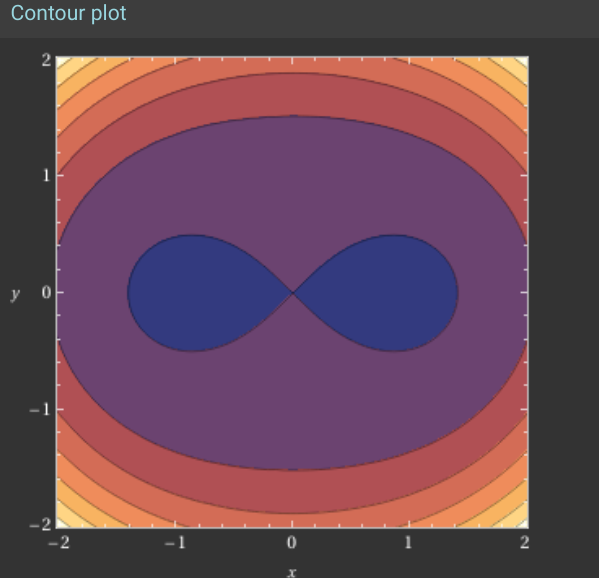
\includegraphics[width=0.3\textwidth]{./contour.png}
	\end{center}
\end{figure}

\end{document}
